\subsection{Gene prediction}

In computational biology gene prediction or gene finding refers to the process
of \textbf{identifying the regions of genomic DNA that encode genes}.

This includes \textbf{protein-coding genes as well as RNA genes}, but may also
include prediction of other functional elements such as regulatory regions.

Gene finding is one of the first and most important steps in understanding
the genome of a species once it has been sequenced.

In its earliest days, ``gene finding'' was based on painstaking experimentation
on living cells and organisms.

Statistical analysis of the rates of homologous recombination of several
different genes could determine their order on a certain chromosome, and
information from many such experiments could be combined to create a genetic
map specifying the rough location of known genes relative to each other.

Today, with comprehensive genome sequence and powerful computational resources
at the disposal of the research community,
gene finding has been redefined as a largely computational problem.

Determining that a sequence is functional should be distinguished from
determining the function of the gene or its product.

Gene prediction is one of the key steps in genome annotation, following
sequence assembly, the filtering of non-coding regions and repeat masking.

The prediction of genetic elements in a genomic sequence is done using
different approaches:

\begin{itemize}
  \item \textbf{De novo predictions} (training set)
  \item \textbf{Evidence based} (EST and proteins)
  \item \textbf{Comparative genomics} (other genomes)
  \item \textbf{RNA-seq} (NGS reads)
  \item \textbf{Combiner} (training set)
\end{itemize}

\paragraph*{GBrowse}

The Gbrowse helps in the understanding of the predictions.

Gbrowse is a tool for the visualization of genetic annotations.

It is based on a relational database (MySQL or Postgres) where all the traces
are stored.

\subsection{DNA annotation}

DNA annotation or genome annotation is the process of identifying the
locations of genes and all of the coding regions in a genome and
\textbf{determining what those genes do}.

An annotation (irrespective of the context) is a note added by way of
explanation or commentary.

Once a genome is sequenced, it needs to be annotated to make sense of it.

For DNA annotation, a previously unknown sequence representation of genetic
material is enriched with information relating genomic position to intron-exon
boundaries, regulatory sequences, repeats, gene names and protein products.

This annotation is stored in genomic databases.

\paragraph{Automatic annotation}

\begin{itemize}
 \item Relatively fast
 \item Large number of annotations derived from sequence similarity and
``mapping files''.
 \item Useful in the preliminary phase of genomic annotation. They provide a
``draft'' of the `` genomic book''
\end{itemize}

\begin{figure}[H]
  \centering
  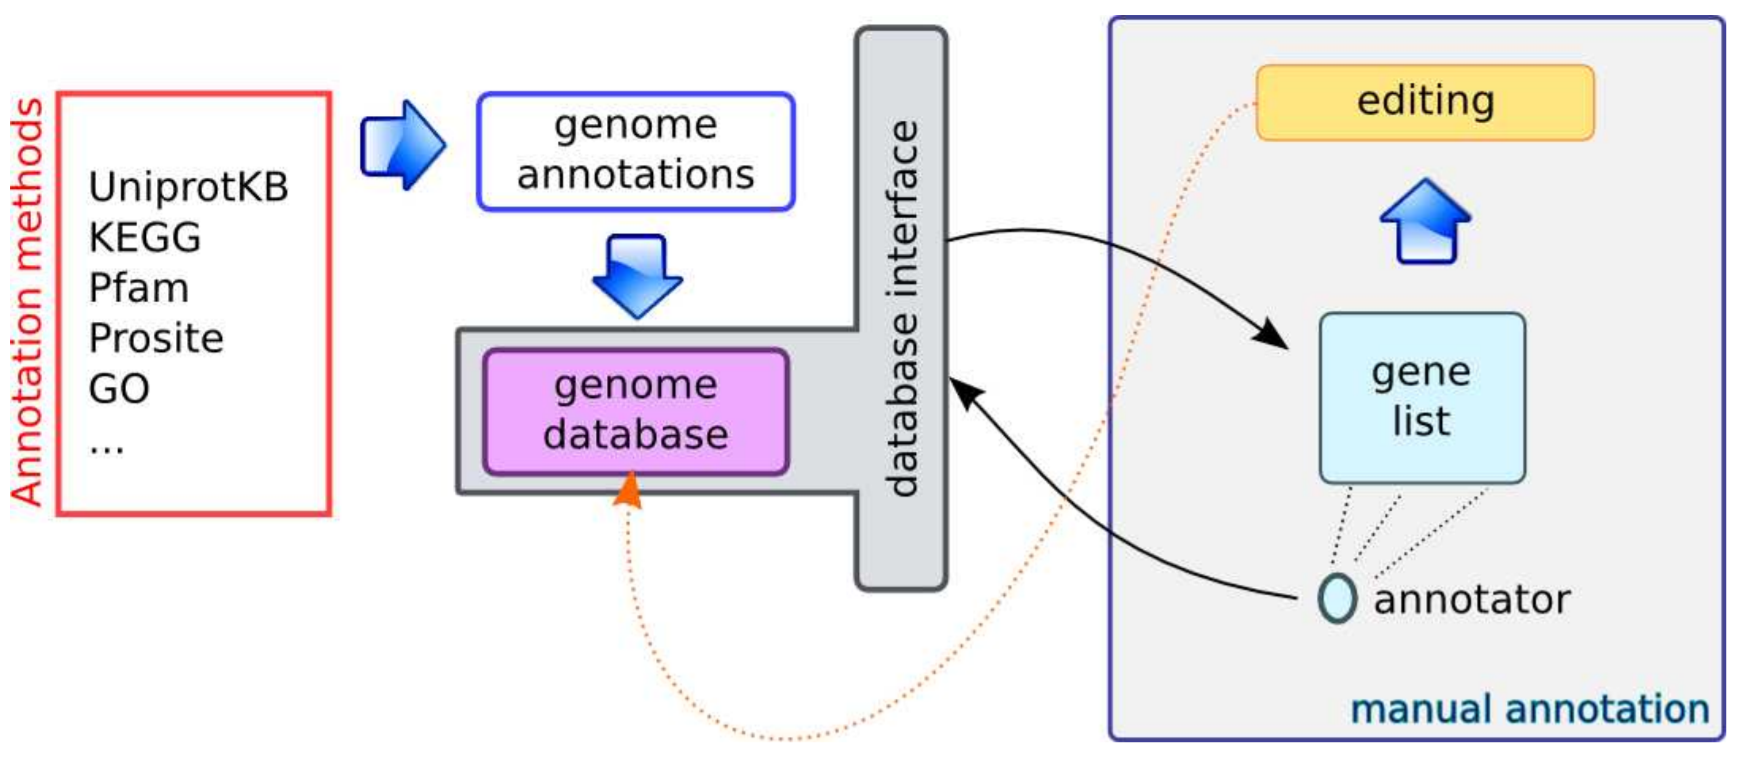
\includegraphics[scale=0.2]{annotation_summary}
  \caption{Genome annotation: summary}
  \label{fig:annotation_summary}
\end{figure}

\subsection{Markov Chain}
With the Markov Chain you can predict the next base after a sequence. In this
way you can have a probabilistic approach to the
problem.\footnote{\url{http://projects.haykranen.nl/markov/demo/}}
